Konstruieren Sie einen Stackautomaten, der die Sprache
\[
L=\{{\tt a}^i{\tt b}^j| i\ne j\}
\]
akzeptiert.

\thema{Stackautomat}

\begin{loesung}
Der PDA funktioniert nach dem gleichen Prinzip wie der in der Vorlesung
besprochene PDA, der die Sprache $\{{\tt 0}^n{\tt 1}^n|n\ge 0\}$
akzeptiert.

Wenn $i>j$ ist, dann ist es am Ende des Wortes noch möglich, mindestens
ein weiteres {\tt a} vom Sack zu lesen, bevor das Stackende-Zeichen
gefunden wird.

Wenn $i<j$ ist, dann kann nach dem erreichen des Stackende-Zeichens
noch ein {\tt b} vom Input gelesen werden, und weitere {\tt b}
können gelesen werden, ohne dass der Stack modifiziert wird.
\begin{center}
\def\l{3}
\def\h{2}
\def\zustand#1#2{
	\draw #1 circle[radius=0.4cm];
	\node at #1 {#2};
}
\def\akzeptierzustand#1#2{
	\zustand{#1}{#2}
	\draw #1 circle[radius=0.35cm];
}
\begin{tikzpicture}[>=latex,thick]
\coordinate (q0) at (0,0);
\coordinate (s) at (-2,0);
\coordinate (q1) at ({1*\l},{0*\h});
\coordinate (q2) at ({2*\l},{0*\h});
\coordinate (q3) at ({2.5*\l},{1*\h});
\coordinate (q4) at ({3.5*\l},{1*\h});
\coordinate (q5) at ({2.5*\l},{-1*\h});
\coordinate (q6) at ({3.5*\l},{-1*\h});
\zustand{(q0)}{$q_0$}
\zustand{(q1)}{$q_1$}
\zustand{(q2)}{$q_2$}
\zustand{(q3)}{$q_3$}
\akzeptierzustand{(q4)}{$q_4$}
\zustand{(q5)}{$q_5$}
\akzeptierzustand{(q6)}{$q_6$}
\draw[->,shorten <= 0.4cm,shorten >= 0.4cm] (s) -- (q0);
\draw[->,shorten <= 0.4cm,shorten >= 0.4cm] (q0) -- (q1);
\draw[->,shorten <= 0.4cm,shorten >= 0.4cm] (q1) -- (q2);
\draw[->,shorten <= 0.4cm,shorten >= 0.4cm] (q2) -- (q3);
\draw[->,shorten <= 0.4cm,shorten >= 0.4cm] (q3) -- (q4);
\draw[->,shorten <= 0.4cm,shorten >= 0.4cm] (q2) -- (q5);
\draw[->,shorten <= 0.4cm,shorten >= 0.4cm] (q5) -- (q6);
\draw[->,shorten <= 0.4cm,shorten >= 0.4cm]
	(q1) to[out=60,in=120,distance=1.4cm] (q1);
\draw[->,shorten <= 0.4cm,shorten >= 0.4cm]
	(q2) to[out=80,in=140,distance=1.4cm] (q2);
\draw[->,shorten <= 0.4cm,shorten >= 0.4cm]
	(q3) to[out=120,in=180,distance=1.4cm] (q3);
\draw[->,shorten <= 0.4cm,shorten >= 0.4cm]
	(q5) to[out=-120,in=-180,distance=1.4cm] (q5);
\node at ($0.5*(q0)+0.5*(q1)$)
	[above] {$\varepsilon,\varepsilon\to\texttt{\$}$};
\node at ($0.5*(q1)+0.5*(q2)$)
	[above] {$\varepsilon,\varepsilon\to\varepsilon$};
\node at ($0.5*(q3)+0.5*(q4)$)
	[above] {$\varepsilon,\texttt{\$}\to\varepsilon$};
\node at ($0.5*(q5)+0.5*(q6)$)
	[below] {$\varepsilon,\varepsilon\to\varepsilon$};
\node at ($(q1)+(0,1.0)$) [above] {$\texttt{a},\varepsilon\to\texttt{a}$};
\node at ($(q2)+(-0.5,1.0)$) [above] {$\texttt{b},\texttt{a}\to\varepsilon$};
\node at ($(q3)+(-0.9,0.3)$) [left] {$\varepsilon,\texttt{a}\to\varepsilon$};
\node at ($(q5)+(-0.9,-0.3)$) [left] {$\texttt{b},\varepsilon\to\varepsilon$};
\node at ($0.5*(q2)+0.5*(q3)$)
	[below right] {$\varepsilon,\texttt{a}\to\varepsilon$};
\node at ($0.5*(q2)+0.5*(q5)$)
	[above right] {$\texttt{b},\texttt{\$}\to\varepsilon$};
\end{tikzpicture}
\end{center}
%\[
%\entrymodifiers={++[o][F]}
%\xymatrix @+5mm{
%*+\txt{}
%        &*+\txt{}
%                &*+\txt{}
%                        &*+\txt{}
%                                &{q_3}\ar@(ur,ul)_{\varepsilon, {\tt a}\to\varepsilon}
%                                 \ar[r]^{\varepsilon,{\tt \$}\to\varepsilon}
%                                        &*++[o][F=]{q_4}
%\\
%*+\txt{}\ar[r]
%        &{q_0}\ar[r]^{\varepsilon,\varepsilon\to{\tt \$}}
%                &{q_1}\ar@(ur,ul)_{{\tt a},\varepsilon\to{\tt a}}
%                   \ar[r]^{\varepsilon,\varepsilon\to\varepsilon}
%                        &{q_2}\ar@(ur,ul)_{{\tt b},{\tt a}\to\varepsilon}
%                           \ar[ur]_{\varepsilon,{\tt a}\to\varepsilon}
%                           \ar[dr]^{{\tt b},{\tt \$}\to\varepsilon}
%\\
%*+\txt{}
%        &*+\txt{}
%                &*+\txt{}
%                        &*+\txt{}
%                                &{q_5}\ar@(dr,dl)^{{\tt b},\varepsilon\to\varepsilon}
%                                       \ar[r]^{\varepsilon,\varepsilon\to\varepsilon}
%                                        &*++[o][F=]{q_6}
%}
%\]

Alternativ könnte man den Stackautomaten dadurch finden, dass man
zuerst eine Grammatik konstruiert, und die dann mit Hilfe des Algorithmus
aus der Vorlesung in einen Stackautomaten umwandelt. Die Grammatik
muss Wörter mit einem "Uberschuss an {\tt a} oder {\tt b}
produzieren, wir schreiben die Variable $A$ für Wörter mit einem
"Uberschuss an {\tt a} und $B$ für Wörter mit einem "Uberschuss an
{\tt b}. Wörter mit einem "Uberschuss an {\tt a} entstehen, in dem man
solche Wörter immer im {\tt a} links wachsen lässt oder wenn man
ein {\tt b} rechts anfügt auch ein {\tt b} links hinzufügt. Die Grammatik
wird damit
\begin{align*}
S&\to A|B\\
A&\to {\tt a}A\\
 &\to {\tt a}A{\tt b}\\
 &\to {\tt a}\\
B&\to B{\tt b}\\
 &\to {\tt a}B{\tt b}\\
 &\to {\tt b}\\
\end{align*}
Die Konstruktion aus der Vorlesung liefert jetzt zunächst das
Gerüst des Automaten
\begin{center}
\begin{tikzpicture}[>=latex,thick]
\coordinate (s) at (-2,0);
\coordinate (q0) at (0,0);
\coordinate (q1) at (3,0);
\coordinate (R) at (6,0);
\coordinate (q2) at (9,0);
\draw (q0) circle[radius=0.4];
\draw (q1) circle[radius=0.4];
\draw (q2) circle[radius=0.4];
\draw (R) circle[radius=0.4];
\node at (R) {$R$};
\draw (q2) circle[radius=0.35];
\draw[->,shorten >= 0.4cm,shorten <= 0.4cm] (s) -- (q0);
\draw[->,shorten >= 0.4cm,shorten <= 0.4cm] (q0) -- (q1);
\draw[->,shorten >= 0.4cm,shorten <= 0.4cm] (q1) -- (R);
\draw[->,shorten >= 0.4cm,shorten <= 0.4cm] (R) -- (q2);
\node at ($0.5*(q0)+0.5*(q1)$)
	[above] {$\varepsilon,\varepsilon\to\texttt{\$}$};
\node at ($0.5*(q1)+0.5*(R)$)
	[above] {$\varepsilon,\varepsilon\to S$};
\node at ($0.5*(R)+0.5*(q2)$)
	[above] {$\varepsilon,\texttt{\$}\to\varepsilon$};
\end{tikzpicture}
\end{center}
dem Zustand $R$ fügt man jetzt entsprechend der Regeln folgende
"Ubergänge hinzu.
Für die Regeln mit $A$ sind es die Übergänge im linken Zustandsdiagramm,
für die Regeln mit $B$ sind es die im rechten:
\begin{center}
\begin{tikzpicture}[>=latex,thick]
\begin{scope}[xshift=-4.3cm]
\coordinate (R) at (0,0);
\coordinate (q0) at (-3,0);
\coordinate (q1) at ({1.5*sqrt(3)},1.5);
\coordinate (q2) at ({1.5*sqrt(3)},-1.5);
\coordinate (q1) at (3.1,1.5);
\coordinate (q2) at (3.1,-1.5);
\draw (R) circle[radius=0.35];
\node at (R) {$R$};
\draw (q1) circle[radius=0.35];
\draw (q2) circle[radius=0.35];
\draw (q0) circle[radius=0.35];
\draw[->,shorten >= 0.35cm,shorten <= 0.35cm] (R) -- (q1);
\draw[->,shorten >= 0.35cm,shorten <= 0.35cm] (q1) -- (q2);
\draw[->,shorten >= 0.35cm,shorten <= 0.35cm] (q2) -- (R);
\draw[->,shorten >= 0.35cm,shorten <= 0.35cm]
	(R) to[out=160,in=20] (q0);
\draw[->,shorten >= 0.35cm,shorten <= 0.35cm]
	(q0) to[out=-20,in=-160] (R);
\draw[->,shorten >= 0.35cm,shorten <= 0.35cm]
	(R) to[out=60,in=120,distance=1.4cm] (R);
\draw[->,shorten >= 0.35cm,shorten <= 0.35cm]
	(R) to[out=-60,in=-120,distance=1.4cm] (R);
\node at ($0.5*(q1)+0.5*(q2)$)
	[right] {$\varepsilon,\varepsilon\to A$\strut};
\node at ($0.1*(R)+0.9*(q1)+(0,-0.1)$)
	[above left] {$\varepsilon,A\to\texttt{b}$\strut};
\node at ($0.1*(R)+0.9*(q2)+(0,0.1)$)
	[below left] {$\varepsilon,\varepsilon\to\texttt{a}$\strut};
\node at ($0.5*(q0)+0.5*(R)+(0,0.25)$)
	[above] {$\varepsilon,A\to A$\strut};
\node at ($0.5*(q0)+0.5*(R)+(0,-0.25)$)
	[below] {$\varepsilon,\varepsilon\to\texttt{a}$\strut};
\node at ($(R)+(0,1.2)$) {$\varepsilon,S\to A$\strut};
\node at ($(R)+(0,-1.2)$) {$\varepsilon, A\to\texttt{a}$\strut};
\end{scope}
\begin{scope}[xshift=0.66cm]
\draw[color=gray] (0,-2) -- (0,2);
\end{scope}
\begin{scope}[xshift=4.3cm]
\coordinate (R) at (0,0);
\coordinate (q0) at (-3,0);
\coordinate (q1) at ({1.5*sqrt(3)},1.5);
\coordinate (q2) at ({1.5*sqrt(3)},-1.5);
\coordinate (q1) at (3.1,1.5);
\coordinate (q2) at (3.1,-1.5);
\draw (R) circle[radius=0.35];
\node at (R) {$R$};
\draw (q1) circle[radius=0.35];
\draw (q2) circle[radius=0.35];
\draw (q0) circle[radius=0.35];
\draw[->,shorten >= 0.35cm,shorten <= 0.35cm] (R) -- (q1);
\draw[->,shorten >= 0.35cm,shorten <= 0.35cm] (q1) -- (q2);
\draw[->,shorten >= 0.35cm,shorten <= 0.35cm] (q2) -- (R);
\draw[->,shorten >= 0.35cm,shorten <= 0.35cm]
	(R) to[out=160,in=20] (q0);
\draw[->,shorten >= 0.35cm,shorten <= 0.35cm]
	(q0) to[out=-20,in=-160] (R);
\draw[->,shorten >= 0.35cm,shorten <= 0.35cm]
	(R) to[out=60,in=120,distance=1.4cm] (R);
\draw[->,shorten >= 0.35cm,shorten <= 0.35cm]
	(R) to[out=-60,in=-120,distance=1.4cm] (R);
\node at ($0.5*(q1)+0.5*(q2)$)
	[right] {$\varepsilon,\varepsilon\to B$\strut};
\node at ($0.1*(R)+0.9*(q1)+(0,-0.1)$)
	[above left] {$\varepsilon,B\to\texttt{b}$\strut};
\node at ($0.1*(R)+0.9*(q2)+(0,0.1)$)
	[below left] {$\varepsilon,\varepsilon\to\texttt{a}$\strut};
\node at ($0.5*(q0)+0.5*(R)+(0,0.25)$)
	[above] {$\varepsilon,B\to \texttt{b}$\strut};
\node at ($0.5*(q0)+0.5*(R)+(0,-0.25)$)
	[below] {$\varepsilon,\varepsilon\to B$\strut};
\node at ($(R)+(0,1.2)$) {$\varepsilon,S\to B$\strut};
\node at ($(R)+(0,-1.2)$) {$\varepsilon, B\to\texttt{b}$\strut};
\end{scope}
\end{tikzpicture}
\end{center}
%\[
%\entrymodifiers={++[o][F]}
%\xymatrix{
%*+\txt{}
%        &\ar@/^/[d]^{\varepsilon,\varepsilon\to {\tt a}}
%\\
%*+\txt{}
%        &{R}    \ar[r]^{\varepsilon,A\to{\tt b}}
%                \ar@/^/[u]^{\varepsilon,A\to A}
%                \ar@(d,dl)^{\varepsilon,A\to{\tt a}}
%                \ar@(l,dl)_{\varepsilon,S\to A}
%                &{}     \ar[r]^{\varepsilon,\varepsilon\to A}
%                        &{}     \ar@/^10pt/[ll]^{\varepsilon,\varepsilon\to{\tt a}}
%}
%\]
%Und für die Regeln mit $B$:
%\[
%\entrymodifiers={++[o][F]}
%\xymatrix{
%*+\txt{}
%        &\ar@/^/[d]^{\varepsilon,\varepsilon\to B}
%\\
%*+\txt{}
%        &{R}    \ar[r]^{\varepsilon,B\to{\tt b}}
%                \ar@/^/[u]^{\varepsilon,B\to {\tt b}}
%                \ar@(d,dl)^{\varepsilon,B\to{\tt b}}
%                \ar@(l,dl)_{\varepsilon,S\to B}
%                &{}     \ar[r]^{\varepsilon,\varepsilon\to B}
%                        &{}     \ar@/^10pt/[ll]^{\varepsilon,\varepsilon\to{\tt a}}
%}
%\]
Zusätzlich braucht es noch die Regeln, die zur Verarbeitung
der Eingabezeichen nötig sind:
\begin{center}
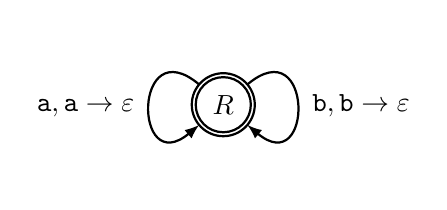
\begin{tikzpicture}[>=latex,thick]
\draw (0,0) circle[radius=0.4];
\draw (0,0) circle[radius=0.35];
\node at (0,0) {$R$};
\draw[->,shorten <= 0.4cm,shorten >= 0.4cm]
	(0,0) to[out=40,in=-40,distance=1.5cm] (0,0);
\draw[->,shorten <= 0.4cm,shorten >= 0.4cm]
	(0,0) to[out=140,in=-140,distance=1.5cm] (0,0);
\node at (1.0,0) [right] {$\texttt{b},\texttt{b}\to\varepsilon$\strut};
\node at (-1.0,0) [left] {$\texttt{a},\texttt{a}\to\varepsilon$\strut};
\end{tikzpicture}
\end{center}
\vspace*{-40pt}
\end{loesung}
